\documentclass[10pt,a4paper]{article}
\usepackage[utf8]{inputenc}
\usepackage[T1]{fontenc}
\usepackage[spanish,es-tabla]{babel}
\usepackage[margin=2.2cm]{geometry}
\usepackage{graphicx,booktabs,tabularx,array,amsmath,xcolor}
\usepackage{hyperref}
\hypersetup{colorlinks=true,urlcolor=blue!45!black,linkcolor=blue!45!black,citecolor=blue!45!black,pdftitle={Ruta 14: visualización de residuos sólidos},pdfauthor={Robert Josue Huanca Clares}}
\setlength{\parindent}{0pt}
\setlength{\parskip}{4pt}
\renewcommand{\arraystretch}{1.18}
\newcolumntype{Y}{>{\raggedright\arraybackslash}X}
\newcommand{\archivo}[1]{\nolinkurl{#1}}
\newcommand{\fuente}[1]{{\footnotesize\textit{Fuente: #1.}}}
\newcommand{\FilasBrutas}{25355}
\newcommand{\FilasProcesadas}{8319}
\newcommand{\Meses}{141}
\newcommand{\MesesCompletos}{141}
\newcommand{\Faltantes}{0}
\newcommand{\Duplicados}{0}
\newcommand{\MesMapa}{2026-09}
\newcommand{\FinFuente}{2026-10}
\begin{document}
\hypersetup{pageanchor=false}
\begin{titlepage}
\centering
{\large UNIVERSIDAD MAYOR DE SAN ANDRÉS\par}
{FACULTAD DE CIENCIAS PURAS Y NATURALES\par}
{CARRERA DE INFORMÁTICA\par}
\vspace{2.6cm}
{\color{blue!35!black}\LARGE\bfseries Visualización de residuos sólidos\par}
\vspace{.5cm}
{\Large Priorización de distritos para campañas de separación y revisión de la recolección\par}
\vspace{.7cm}
{\large Ruta 14 -- Residuos sólidos\par}
{Informe de avance: primera y segunda semana\par}
\vspace{2cm}
\begin{tabular}{rl}
\textbf{Estudiante:} & Robert Josue Huanca Clares \\
\textbf{Asignatura:} & Visualización de Datos (DAT-382) \\
\textbf{Docente:} & M.Sc. Elizabeth Pommier Gallo \\
\textbf{Gestión:} & II -- 2026 \\
\textbf{Fecha:} & 6 de noviembre de 2026
\end{tabular}
\vfill
{La Paz -- Bolivia\par}
\end{titlepage}
\hypersetup{pageanchor=true}

\section*{Primera semana}
\section{Introducción}
Decidir dónde reforzar una campaña de separación requiere algo más que conocer cuánta basura recoge una ciudad. Es necesario observar qué distritos concentran mayores volúmenes, qué materiales se recolectan por separado y cómo cambian estos valores. Una visualización permite revisar esas diferencias sin recorrer miles de filas.

Este proyecto desarrolla una base de datos integrada y un producto visual sobre los 59 distritos comunitarios de Nueva York. Está dirigido a personal de planificación del aseo municipal y, como audiencia secundaria, a juntas vecinales. Combina un mapa, comparaciones entre distritos y una serie mensual. En esta entrega se ejecutan la descarga, el ETL y las figuras; el tablero interactivo y la evaluación con usuarios corresponden a la siguiente etapa.

\section{Antecedentes y elección de los datos}
El acta inicial de la Ruta 14 propone usar datos del Department of Sanitation de Nueva York (DSNY) ante la dificultad de encontrar una serie equivalente por distrito de La Paz~\cite{acta}. La consulta al INE confirma que existe información boliviana sobre recolección por ciudad y procedencia~\cite{ine}. Por tanto, el problema no es una ausencia total de datos locales, sino su adecuación a la unidad de análisis requerida.

\begin{center}\small
\begin{tabularx}{\linewidth}{@{}p{2.7cm}YYY@{}}
\toprule
\textbf{Alternativa} & \textbf{Aporte disponible} & \textbf{Límite para este trabajo} & \textbf{Decisión} \\\midrule
INE, Bolivia & Estadísticas de recolección por ciudad y procedencia. & En las fuentes revisadas no se verificó una serie distrito-mes con papel y MGP. & Contexto; no alimenta el cálculo. \\
Reportes de La Paz & Diagnósticos sobre residuos y economía circular~\cite{lapaz}. & Un informe no sustituye una tabla mensual descargable con claves territoriales compatibles. & Antecedente local. \\
DSNY + DCP, NYC & Tonelaje mensual, geometría y población histórica por distrito. & Contexto distinto; población desactualizada para tasas actuales. & Caso de aplicación reproducible. \\
\bottomrule
\end{tabularx}\end{center}
\fuente{consulta de fuentes institucionales y evaluación propia, 06-11-2026}

Esta elección permite practicar un método transferible a La Paz, pero no trasladar sus cifras ni sus prioridades. La búsqueda descrita tampoco demuestra que ninguna institución paceña tenga registros más detallados: se necesitaría solicitarlos y comprobar su cobertura.

\section{Planteamiento del problema}
Las tablas de tonelaje, los límites geográficos y la población se publican por separado. Sin integrarlos y precisar qué mide cada variable, resulta difícil distinguir una alta carga de recolección de una baja proporción de materiales separados. Esto puede llevar a priorizar campañas con comparaciones incompletas o atribuir al comportamiento ciudadano diferencias que dependen del servicio.

\textbf{Pregunta del problema:} ¿Qué diferencias territoriales y temporales presenta la recolección de basura común, papel y MGP en los distritos de Nueva York entre enero de 2015 y septiembre de 2026, y qué distritos requieren una revisión prioritaria de sus necesidades de separación y recolección?

\newpage
\section{Objetivos}
\subsection{Objetivo general}
Implementar una solución de visualización de datos que apoye la priorización de distritos para campañas de separación y revisión de la recolección, mediante el análisis del tonelaje mensual de Nueva York entre enero de 2015 y septiembre de 2026.

\subsection{Objetivos específicos}
\begin{enumerate}
\item Analizar el problema, la cobertura de las fuentes y las necesidades de información del personal de planificación municipal.
\item Diseñar y ejecutar un proceso ETL reproducible que integre los datos por distrito y mes, conservando su procedencia y verificando su calidad.
\item Desarrollar indicadores, un mapa y gráficos de comparación y evolución que sirvan de base al tablero de la Ruta 14.
\item Verificar la consistencia de los resultados y evaluar la usabilidad, accesibilidad y utilidad del producto con tareas de consulta definidas.
\end{enumerate}

\section{Marco conceptual, normativo y metodológico}
\subsection{Visualización, percepción y narrativa}
La visualización relaciona datos con posiciones, formas y colores para facilitar comparaciones. La narrativa de este proyecto sigue tres preguntas: \textit{¿dónde hay diferencias?, ¿qué magnitud tienen?, ¿cómo evolucionan?} Cada autor orienta una decisión concreta, en lugar de incorporarse solo como referencia teórica.

\begin{center}\small
\begin{tabularx}{\linewidth}{@{}p{3.7cm}Y@{}}
\toprule
\textbf{Referencia} & \textbf{Aplicación al proyecto} \\\midrule
Bertin~\cite{bertin} & Usar una escala secuencial de color para ordenar proporciones en el mapa. \\
Cleveland y McGill~\cite{cleveland} & Complementar el mapa con barras sobre un eje común para comparar valores con precisión. \\
Munzner~\cite{munzner} & Separar necesidad del usuario, tarea analítica, codificación visual e implementación; comprobar cada nivel. \\
Few~\cite{few} & Reunir pocos indicadores pertinentes y evitar elementos decorativos que dificulten la lectura. \\
Tufte~\cite{tufte} & Mantener escalas, unidades y fuentes visibles; evitar efectos 3D y distorsiones de magnitud. \\
Ware~\cite{ware} & Utilizar contraste y agrupación visual, sin depender únicamente del color para comunicar valores. \\
Shneiderman~\cite{shneiderman} & Diseñar el futuro tablero con vista general, filtros de periodo y distrito, y detalle bajo demanda. \\
\bottomrule
\end{tabularx}\end{center}

\subsection{Marcos de trabajo}
\textbf{CRISP-DM} organiza comprensión del problema, comprensión y preparación de datos, análisis, evaluación y despliegue~\cite{crisp}. Aquí la fase de modelado se adapta al cálculo de indicadores; no se necesita un modelo predictivo. El \textbf{modelo anidado de Munzner} ayuda a comprobar que una gráfica correcta responda a una pregunta útil. \textbf{PDCA} ordena la mejora: planificar criterios, ejecutar el ETL, comprobar resultados y corregir. \textbf{ISO 31000:2018} orienta la identificación y tratamiento de riesgos~\cite{risk}: población antigua, cambios de definición y confusión entre recolección y reciclaje efectivo.

\newpage
\subsection{Normas y evidencia de aplicación}
Se incluyen las familias ISO/IEC e IEEE solicitadas en el temario y la norma ambiental focal del acta. Se aplican como referencias para decisiones y controles; este trabajo no constituye una auditoría ni acredita cumplimiento integral o certificación.

\begin{center}\small
\begin{tabularx}{\linewidth}{@{}p{4.0cm}Y@{}}
\toprule
\textbf{Norma} & \textbf{Aplicación y evidencia} \\\midrule
ISO 14001:2026~\cite{ambiental} & Marco de gestión ambiental y mejora continua. Se define un indicador con alcance explícito; la norma no establece el porcentaje calculado ni un umbral de buen desempeño. \\
ISO/IEC 25012:2008~\cite{calidad} & Calidad de datos: completitud, consistencia y trazabilidad. Evidencia: informe JSON, cobertura por mes, claves únicas y validación de tipos. \\
ISO/IEC 27001:2022~\cite{seguridad} & Integridad y disponibilidad: originales separados, hashes SHA-256 y código reproducible. Estos controles locales no equivalen a un sistema de gestión certificado. \\
ISO/IEC 27701:2025~\cite{privacidad} & Referencia de privacidad. Las fuentes usadas son agregadas; no se incorporan identificadores personales ni cruces por domicilio. \\
ISO 9241-210:2019~\cite{usuario} & Diseño centrado en las personas: definir audiencia y tareas. La prueba con usuarios está planificada, aún no ejecutada. \\
IEEE 1012-2024~\cite{ieee} & Distinguir verificación del cálculo y validación de utilidad. Se ejecutan aserciones del ETL; queda pendiente validar decisiones con usuarios. \\
\bottomrule
\end{tabularx}\end{center}

\section*{Segunda semana}
\section{Metodología de desarrollo}
\begin{enumerate}
\item \textbf{Comprender:} precisar la decisión y limitar el alcance a distrito-mes. Sin recorridos, horarios ni capacidad de camiones, no se optimizan rutas individuales.
\item \textbf{Obtener y revisar:} descargar las tres fuentes, sus metadatos y el diccionario DSNY. Revisar definiciones antes de elegir las fracciones comparables.
\item \textbf{Preparar e integrar:} estandarizar fechas y códigos; detectar nulos, duplicados y meses ausentes; unir tablas y geometrías con controles de cardinalidad.
\item \textbf{Analizar y diseñar:} calcular proporciones y volúmenes, elaborar mapa, barras y serie. Comparar distritos en un mismo mes completo para evitar coberturas desiguales.
\item \textbf{Evaluar y desplegar:} comprobar resultados y exportar CSV y GeoJSON. Después, montar el tablero en Power BI y evaluar tareas con usuarios; QGIS puede utilizar la capa ya preparada.
\end{enumerate}

\begin{center}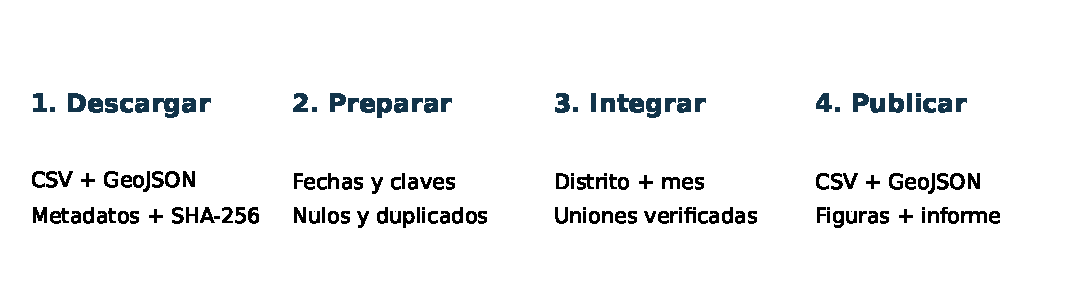
\includegraphics[width=\linewidth]{figures/flujo_etl.pdf}\end{center}

\newpage
\section{Datos y proceso ETL}
\subsection{Fuentes, descarga y condiciones de uso}
Se descargaron las fuentes previstas en el acta~\cite{tonnage,districts,population}. El manifiesto local conserva URL exacta, instante de descarga, tamaño en bytes y hash; no se presentan tamaños o cantidades del acta como si fueran resultados nuevos.

\begin{center}\small
\begin{tabularx}{\linewidth}{@{}p{3.0cm}p{3.5cm}Y@{}}
\toprule
\textbf{Conjunto / ID} & \textbf{Estructura observada} & \textbf{Uso y justificación} \\\midrule
DSNY Monthly Tonnage Data\newline\archivo{ebb7-mvp5} & CSV, \FilasBrutas{} filas, 12 columnas; actualización mensual. & Hecho principal: cantidades por distrito y mes. Se conserva el archivo íntegro y se filtra el periodo del estudio. \\
Community Districts\newline\archivo{5crt-au7u} & GeoJSON, 71 geometrías; clave \archivo{boro_cd}. & Base del mapa. Coinciden 59 distritos con tonelaje; 12 áreas no tienen observación y se mantienen en gris. \\
NYC Population By Community Districts\newline\archivo{xi7c-iiu2} & CSV, 59 filas, 8 columnas; censos 1970--2010. & Nombres de distritos y contexto histórico. No se usa para calcular residuos por habitante en 2015--2026. \\
\bottomrule
\end{tabularx}\end{center}

Las descargas de CSV utilizan el endpoint de exportación completa; la capa se obtiene como GeoJSON. También se guarda el diccionario oficial adjunto, versión 16-04-2026. Las consultas realizadas no necesitaron registro ni token. La configuración admite un token opcional, pero no contiene credenciales.

\textbf{Licencia:} se documentan los términos de uso de NYC Open Data, no se atribuye una licencia Creative Commons que no fue verificada~\cite{terms}. El portal advierte que los datos pueden actualizarse y no garantiza su adecuación a cada uso. Por eso se conservan las copias originales y se distingue entre datos institucionales y cálculos propios.

\subsection{Diccionario de variables utilizadas}
\begin{center}\small
\begin{tabularx}{\linewidth}{@{}p{4.5cm}Y@{}}
\toprule
\textbf{Campo original / derivado} & \textbf{Significado y tratamiento} \\\midrule
\archivo{MONTH} & Texto \archivo{YYYY / MM}; se convierte al primer día del mes. \\
\archivo{BOROUGH}, \archivo{BOROUGH_ID},\newline\archivo{COMMUNITYDISTRICT} & Borough, código y distrito; forman una clave territorial única. El número de distrito solo no identifica el territorio. \\
\archivo{REFUSETONSCOLLECTED} & Basura común; se renombra \archivo{basura}. Incluye recolección de residencias e instituciones. \\
\archivo{PAPERTONSCOLLECTED} & Papel recolectado por separado; se renombra \archivo{papel}. \\
\archivo{MGPTONSCOLLECTED} & Metal, vidrio, plástico y cartones de bebidas agrupados; se renombra \archivo{mgp}. \\
\archivo{boro_cd}, geometría & Código territorial y polígonos para la unión espacial. El mapa se proyecta a EPSG:2263. \\
\texttt{CD Name}, \texttt{2010 Population} & Nombre y población censal histórica; se conservan como atributos contextuales. \\
\bottomrule
\end{tabularx}\end{center}
Se mantiene la unidad publicada, \textit{tons DSNY}, sin convertirla ni equipararla a toneladas métricas. El diccionario completo de campos y tipos queda en \archivo{data/processed/diccionario_fuentes.csv}. Los cinco campos de orgánicos se conservan en bruto, pero se excluyen del análisis distrital según el alcance y las limitaciones operativas descritas por DSNY.

\newpage
\subsection{Reglas de limpieza, integración y carga}
\begin{center}\small
\begin{tabularx}{\linewidth}{@{}p{2.7cm}YY@{}}
\toprule
\textbf{Paso} & \textbf{Regla aplicada} & \textbf{Por qué se aplica} \\\midrule
Conservar & Separar \archivo{raw/} de \archivo{processed/}; verificar hashes. & Poder reconstruir el cálculo sin alterar el origen. \\
Filtrar & Enero de 2015 a septiembre de 2026, ambos incluidos. & Respetar el acta; la fuente ya contiene \FinFuente{}, que queda fuera. \\
Normalizar & Convertir fechas y números de forma estricta. Clave: $100\times\text{borough ID}+\text{distrito}$. & Evitar fechas ambiguas y uniones entre distritos homónimos. \\
Depurar & Eliminar solo duplicados exactos; detener si una clave distrito-mes tiene valores contradictorios. & No elegir arbitrariamente un registro ni sumar dos veces. \\
Controlar & Conservar nulos, rechazar negativos y registrar meses ausentes. & Un dato faltante no representa cero recolección. \\
Integrar & Unión muchos-a-uno con población y uno-a-uno con geometría para el mes del mapa. & Evitar multiplicar filas o perder distritos al unir. \\
Cargar & Exportar CSV, GeoJSON y controles de calidad. & Reutilizar el mismo resultado en notebooks, QGIS, Power BI y LaTeX. \\
\bottomrule
\end{tabularx}\end{center}

\subsection{Definición del indicador}
Para un distrito y mes, sean $B$ la basura común, $P$ el papel y $M$ el MGP:
\[
S=100\,\frac{P+M}{B+P+M}.
\]
Se denomina \textbf{proporción de papel y MGP en las tres fracciones recolectadas}. No mide reciclaje efectivo, contaminación de materiales ni toda la separación, porque excluye orgánicos. Si falta una fracción o el denominador es cero, el resultado queda sin dato. Al agregar distritos o meses se dividen las sumas de masas; no se promedian porcentajes.

Se propone una señal exploratoria: basura común en el cuartil superior y proporción $S$ en el cuartil inferior del mismo mes. Es una forma transparente de seleccionar casos para revisar, no un umbral normativo. Un volumen alto puede reflejar población, instituciones o cobertura del servicio.

\subsection{Resultados de calidad y evidencia ejecutada}
El filtro produjo \textbf{\FilasProcesadas{} registros}: 59 distritos por \Meses{} meses. Se verificaron \MesesCompletos{} meses completos, \Faltantes{} combinaciones ausentes y \Duplicados{} duplicados exactos. No se encontraron claves contradictorias, valores negativos ni nulos en las tres fracciones analizadas. Por ello, no fue necesario imputar ni eliminar registros por esos motivos.

Los tres notebooks de la carpeta \archivo{notebooks/} documentan la descarga, la integración y las figuras, con código y salidas reales. La ejecución fue local en Python, no en Google Colab. Las evidencias son las tablas, controles y figuras guardadas; no se simulan capturas de una herramienta que no se utilizó.

\newpage
\subsection{Evidencia visual e interpretación}
\begin{figure}[h!]
\centering
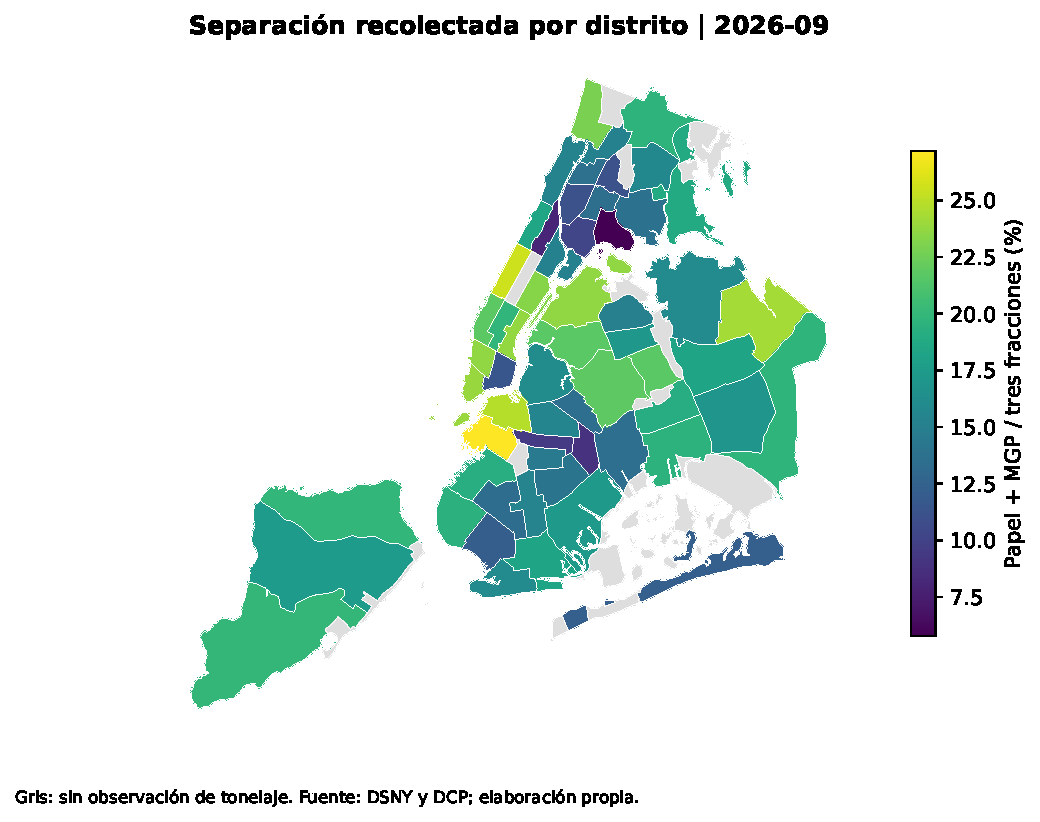
\includegraphics[width=.80\linewidth]{figures/mapa_separacion.pdf}
\caption{Mapa del último mes completo dentro del alcance: \MesMapa{}. Las áreas grises no tienen observación de tonelaje. Fuente: DSNY y DCP; elaboración propia.}
\end{figure}

El mapa responde al visual obligatorio de la Ruta 14. Usa proporciones para que el color no represente simplemente el tamaño de la población o del distrito. Aun así, no controla diferencias en cobertura del servicio o composición de los residuos. Las barras permiten comprobar las diferencias que el color solo aproxima.

\begin{figure}[h!]
\centering
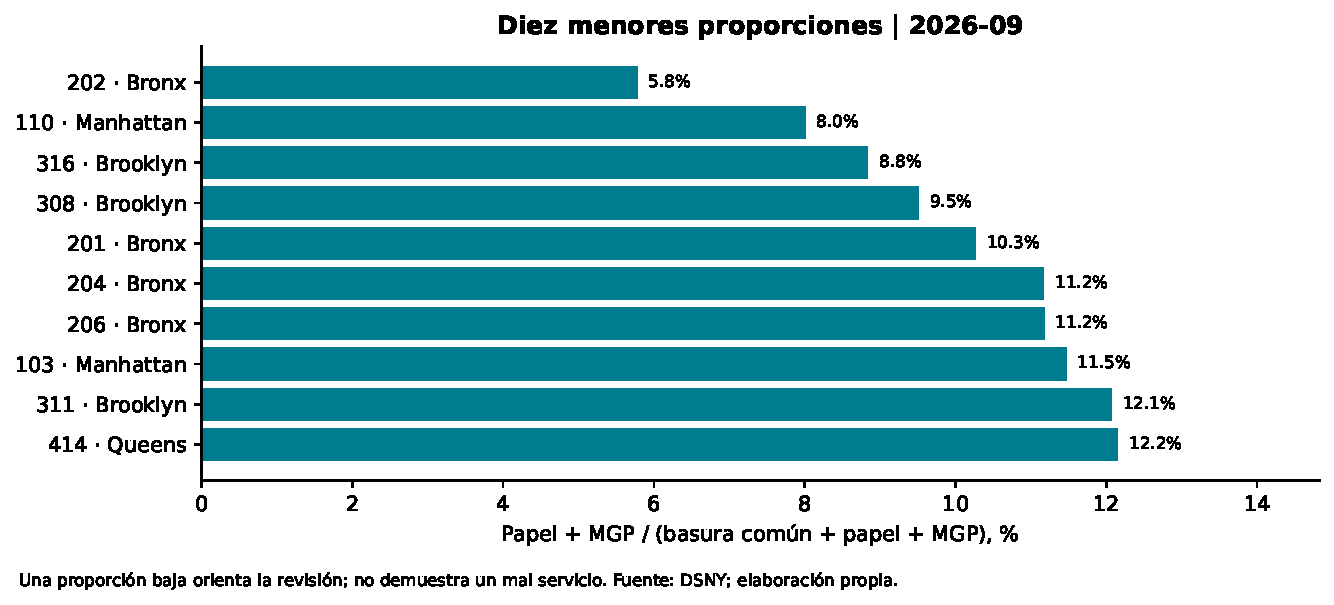
\includegraphics[width=.86\linewidth]{figures/comparacion_distritos.pdf}
\caption{Comparación de las diez menores proporciones en el mismo mes. Los códigos identifican de forma única cada distrito. Fuente: DSNY; elaboración propia.}
\end{figure}

\newpage
\begin{figure}[h!]
\centering
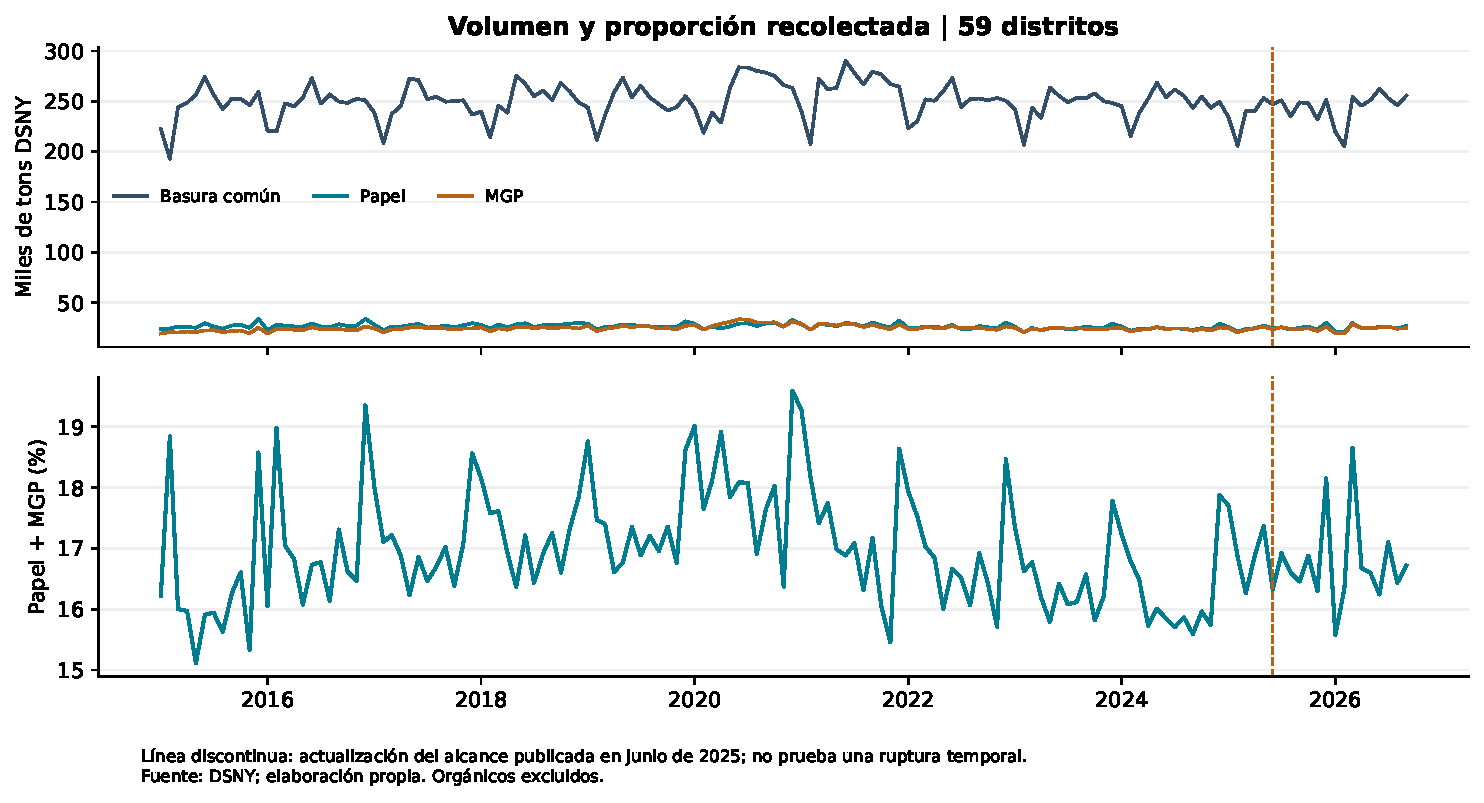
\includegraphics[width=\linewidth]{figures/serie_mensual.pdf}
\caption{Evolución del volumen y de la proporción agregada. Se mantienen las unidades de origen. Fuente: DSNY; elaboración propia.}
\end{figure}

La serie permite formular preguntas sobre cambios y patrones mensuales, pero no demuestra estacionalidad por sí sola. El diccionario informa que la actualización de junio de 2025 amplió los códigos incluidos en basura, papel y MGP. La marca en el gráfico identifica esa actualización; no asegura que el cambio se aplicara solo desde ese mes ni descarta revisiones históricas. Antes de atribuir variaciones a campañas o hábitos se debe revisar esta comparabilidad.

En \MesMapa{}, el criterio de cuartiles selecciona los códigos \textbf{103, 110, 202, 305, 308, 311 y 312}. Son casos para revisar junto con personal municipal, no una lista definitiva de distritos con mal servicio. El detalle está en \archivo{comparacion_ultimo_mes.csv}.

\subsection{Evaluación pendiente y alcance de la entrega}
La verificación técnica ya comprueba conservación de totales, claves, cobertura, geometrías y casos límite del indicador. Para validar el tablero se proponen tres tareas: localizar un distrito con baja proporción, comparar dos meses y explicar qué significa un área gris. Con al menos tres participantes de perfil afín se registrarán aciertos, tiempo, dificultades y sugerencias; como criterio inicial, cada participante deberá resolver al menos dos tareas y ninguno deberá confundir ausencia con cero.

La revisión de accesibilidad comprobará etiquetas legibles, contraste, navegación por teclado en el tablero y una tabla alternativa al mapa. Las figuras actuales tienen leyendas y unidades, pero todavía no se ha probado su comprensión con usuarios. La utilidad se evaluará preguntando qué decisión pueden apoyar y qué información adicional necesitarían antes de actuar.

Se entregan el entorno, los datos originales y procesados, los notebooks y las figuras. No se ha construido un archivo Power BI ni ejecutado una prueba en QGIS. Tampoco se estiman rutas de camiones, tasas actuales por habitante o impactos de una campaña. Estos límites mantienen coherencia entre los datos disponibles y las conclusiones que pueden sostenerse.

\newpage
\small
\begin{thebibliography}{99}
\setlength{\itemsep}{3pt}
\bibitem{acta} Huanca Clares, R. J. (2026). \textit{Ruta 14 -- Residuos sólidos. Acta de alcance individual}. Documento base: \archivo{proy-visualizacion.pdf}.
\bibitem{ine} INE Bolivia. \textit{Residuos sólidos: introducción y cuadros estadísticos}. \href{https://www.ine.gob.bo/index.php/medio-ambiente/residuos-solidos-introduccion/}{Descripción institucional}; \href{https://www.ine.gob.bo/index.php/medio-ambiente/residuos-solidos-cuadros-estadisticos/}{cuadros disponibles}.
\bibitem{lapaz} Gobierno Autónomo Municipal de La Paz. \textit{Residuos y economía circular: oportunidades para emprender}. \href{https://lapaz.bo/wp-content/uploads/2025/01/Residuos-y-economia-circular_-oportunidades-para-emprender-1.pdf}{Documento institucional}.
\bibitem{tonnage} DSNY. \textit{DSNY Monthly Tonnage Data}, ID ebb7-mvp5, y diccionario adjunto de 16-04-2026. \url{https://data.cityofnewyork.us/d/ebb7-mvp5}.
\bibitem{districts} DCP. \textit{Community Districts}, ID 5crt-au7u. \url{https://data.cityofnewyork.us/d/5crt-au7u}.
\bibitem{population} DCP. \textit{New York City Population By Community Districts}, ID xi7c-iiu2. \url{https://data.cityofnewyork.us/d/xi7c-iiu2}.
\bibitem{terms} NYC Open Data. \textit{Terms of Use}. \url{https://data.cityofnewyork.us/stories/s/Terms-of-Use/k9k7-3cje}.
\bibitem{bertin} Bertin, J. (1967). \textit{Sémiologie graphique}. Gauthier-Villars / Mouton.
\bibitem{cleveland} Cleveland, W. S. y McGill, R. (1984). Graphical perception: theory, experimentation, and application to the development of graphical methods. \textit{JASA}, 79(387), 531--554. \url{https://doi.org/10.1080/01621459.1984.10478080}.
\bibitem{munzner} Munzner, T. (2009). A nested model for visualization design and validation. \textit{IEEE TVCG}, 15(6), 921--928. \url{https://www.cs.ubc.ca/labs/imager/tr/2009/NestedModel/}.
\bibitem{few} Few, S. (2013). \textit{Information Dashboard Design}, 2.ª ed. Analytics Press. \url{https://analyticspress.com/idd.php}.
\bibitem{tufte} Tufte, E. R. (2001). \textit{The Visual Display of Quantitative Information}, 2.ª ed. Graphics Press.
\bibitem{ware} Ware, C. (2013). \textit{Information Visualization: Perception for Design}, 3.ª ed. Morgan Kaufmann.
\bibitem{shneiderman} Shneiderman, B. (1996). The eyes have it: a task by data type taxonomy for information visualizations. \textit{IEEE Symposium on Visual Languages}, 336--343. \url{https://www.cs.umd.edu/users/ben/papers/Shneiderman1996eyes.pdf}.
\bibitem{crisp} IBM. \textit{CRISP-DM Help Overview}. \url{https://www.ibm.com/docs/en/spss-modeler/saas?topic=dm-crisp-help-overview}.
\bibitem{ambiental} ISO. \textit{ISO 14001:2026: Environmental management systems}. \url{https://www.iso.org/standard/14001}.
\bibitem{calidad} ISO/IEC. \textit{25012:2008: Data quality model}. \url{https://www.iso.org/standard/35736.html}.
\bibitem{seguridad} ISO/IEC. \textit{27001:2022: Information security management systems}. \url{https://www.iso.org/standard/27001}.
\bibitem{privacidad} ISO/IEC. \textit{27701:2025: Privacy information management systems}. \url{https://www.iso.org/standard/27701}.
\bibitem{usuario} ISO. \textit{9241-210:2019: Human-centred design for interactive systems}. \url{https://www.iso.org/standard/77520.html}.
\bibitem{ieee} IEEE. \textit{1012-2024: System, Software, and Hardware Verification and Validation}. \url{https://standards.ieee.org/ieee/1012/7324/}.
\bibitem{risk} ISO. \textit{31000:2018: Risk management -- Guidelines}. \url{https://www.iso.org/standard/31000}.
\end{thebibliography}
\footnotesize Consulta de fuentes web: 6 de noviembre de 2026. Las normas se documentan mediante sus fichas oficiales; no se reproduce ni se afirma haber auditado su texto íntegro.
\end{document}
